\documentclass[11pt,a4paper]{article}
\usepackage[utf8]{inputenc}
\usepackage{amsmath}
\usepackage{mathtools}
\usepackage{amsfonts}
\usepackage{amssymb}
\usepackage{graphicx}
\usepackage{caption}
\usepackage{subcaption}
\usepackage{comment}
\usepackage{color}
\usepackage{enumitem}
\usepackage[left=2cm,right=2cm,top=2cm,bottom=2cm]{geometry}
\usepackage{listings}
\usepackage{color}

\setlength{\jot}{10pt}
 
\definecolor{codegreen}{rgb}{0,0.6,0}
\definecolor{codegray}{rgb}{0.5,0.5,0.5}
\definecolor{codepurple}{rgb}{0.58,0,0.82}
\definecolor{backcolour}{rgb}{0.95,0.95,0.92}
 
\lstdefinestyle{mystyle}{
    backgroundcolor=\color{backcolour},   
    commentstyle=\color{codegreen},
    keywordstyle=\color{magenta},
    numberstyle=\tiny\color{codegray},
    stringstyle=\color{codepurple},
    basicstyle=\footnotesize,
    breakatwhitespace=false,         
    breaklines=true,                 
    captionpos=b,                    
    keepspaces=true,                 
    numbers=left,                    
    numbersep=5pt,                  
    showspaces=false,                
    showstringspaces=false,
    showtabs=false,                  
    tabsize=2
}
 
\lstset{style=mystyle}
\author{Andrew Teta}
\title{ECEN 4532 - Lab 3: Perspective Transformations and Motion Tracking}
\date{February 25, 2019}

\begin{document}

\maketitle

\begin{figure}[ht]
	\centering
	\begin{subfigure}[h]{0.6\textwidth}
		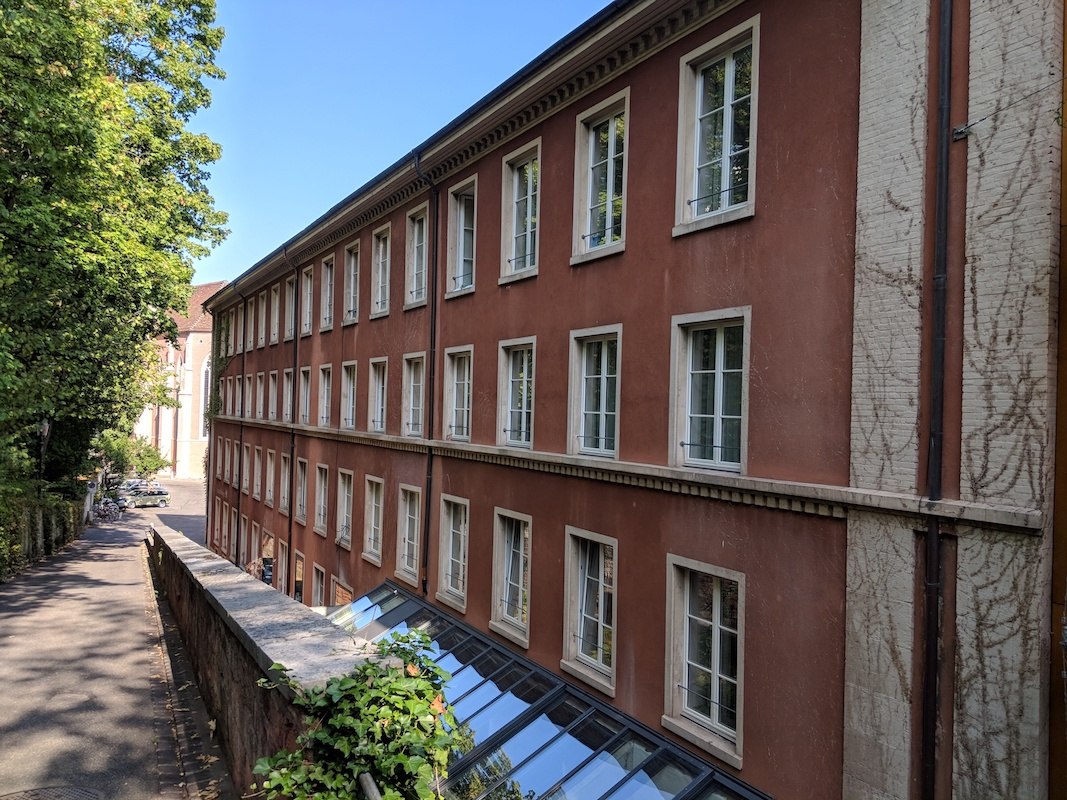
\includegraphics[width=\textwidth]{PC_test_2}
	\end{subfigure}
	\par\bigskip
	\begin{subfigure}[h]{0.6\textwidth}
		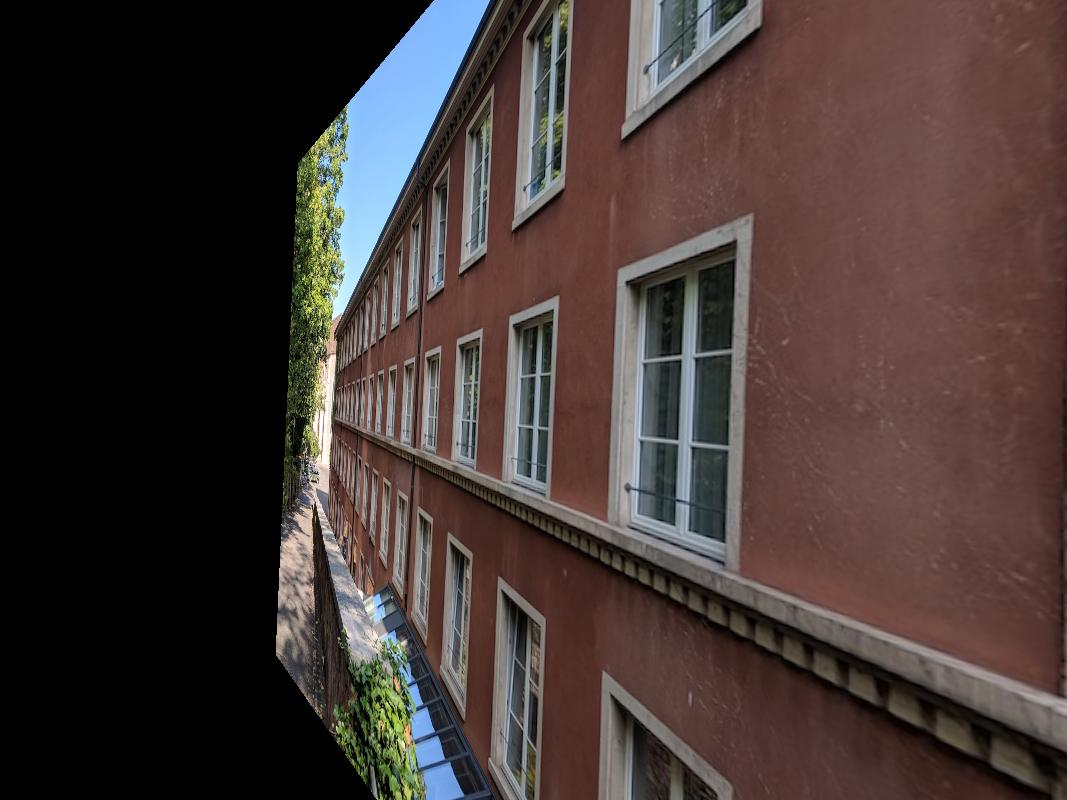
\includegraphics[width=\textwidth]{out1}
	\end{subfigure}
\end{figure}

\pagebreak

\tableofcontents

\pagebreak

\addcontentsline{toc}{section}{Introduction}
\section{Introduction}
In this lab, we explore the low-level implementation of perspective distortion correction, and a simplified model of video motion tracking between frames in Python. We will mostly use \verb|numpy| to manipulate N-D arrays of pixel information. Additionally, I used a free photo editing software called GIMP to select pixel indexes.

\subsection{Background}
Our algorithm for perspective distortion correction relies on the math theory of linear algebra, using a linear transformation matrix to map pixels from one image to another. The process of motion tracking between frames will be based on a series of image pyramids, using block-based motion estimation to "search" for a matching region in the next frame.

\section{Perspective Distortion Correction}
\subsection{Linear Regression}
We begin by defining linear regression as one approach to modeling the relationship between a set of dependent and independent variables. This method is commonly used to fit a model to an \textbf{over-determined} set of data points. By over-determined, we mean there are more equations defining the data set than there are variables, often occurring when many measurements are performed to estimate a small number of parameters. 

Mathematically, we have a relationship of the form, $Ax=c$, where A is over-determined. This only has a solution if \textbf{c} lies in the column space of A, however there will not be an exact solution if A is over-determined and we instead seek an \textbf{x} that minimizes the mean-squared-error (MSE), defined as, $E=|A\textbf{x}-\textbf{b}|^2$. Ultimately, we want to find a "pseudo-inverse", $A^+$, such that $\textbf{x}^\$=A^+\textbf{c}$.

For a given point, $\textbf{c}$, we want to find the closest point in the column space of A. This turns out to be the projection, $\textbf{p}$, of $\textbf{c}$ onto the column space. Thus, the error is the distance vector, $\textbf{c} - \textbf{p}$, orthogonal to the column space. To be orthogonal, the error vector must be orthogonal to every column of A.

\begin{align*}
(\textbf{c} - \textbf{p})^T A &= \textbf{0} \\
\textbf{p}^T A &= \textbf{c}^T A \\
A^T\textbf{p} &= A^T\textbf{c}
\end{align*}

We are in search of $\textbf{x}^\$$ such that $A\textbf{x}^\$ = \textbf{p}$. Assuming the columns of A are linearly independent and substituting, we obtain

\begin{align*}
A^T A\textbf{x}^\$ &= A^T\textbf{c} \\
\textbf{x}^\$ &= (A^T A)^{-1} A^T\textbf{c}
\end{align*}

Therefore,

\begin{equation} \label{eq:pseudo_inverse}
A^+ = (A^T A)^{-1} A^T
\end{equation}

\pagebreak

To demonstrate linear regression, we consider a hypothetical experiment trying to correlate electrode sensor data to a subjective hunger measurement. The data is as follows.

\begin{figure}[ht]
	\centering
	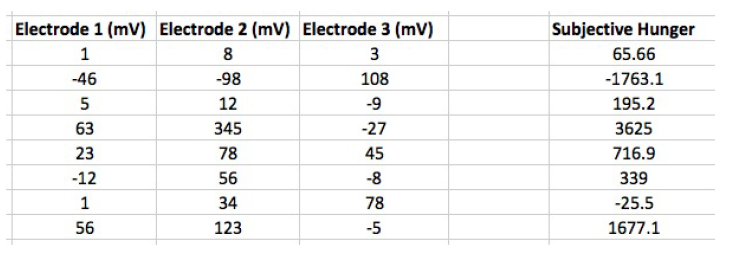
\includegraphics[width = 0.7\textwidth]{electrode}
	\caption{Experimental data}
	\label{fig:electrode}
\end{figure}

In Python, $A_p = A^+$ can be written as \verb|A_p = np.linalg.inv(A.T.dot(A)).dot(A.T)| and calculating $\textbf{x}^\$$, \verb|x = A_p.dot(c)|, the prediction coefficients, we have

\begin{equation}
	x^\$ =
	\begin{bmatrix}
		x1 \\
		x2 \\
		x3
	\end{bmatrix}
	=
	\begin{bmatrix}
		11.93 \\
		8.02 \\
		-3.98
	\end{bmatrix}
\end{equation}

Calculating the MSE for this prediction vector is simple, and results in

\begin{equation}
	MSE = 
	\begin{bmatrix}
	2.36 \\
	2.31 \\
	12.22 \\
	0.05 \\
	13.41 \\
	1.73 \\
	0.36 \\
	8.56
	\end{bmatrix}
\end{equation}

\pagebreak

\subsection{Perspective Correction}
We will use the concept of linear regression to correct perspective distortion in an image. Consider the following diagrams representing a simple model for imaging and projection.

\begin{figure}[ht]
	\centering
	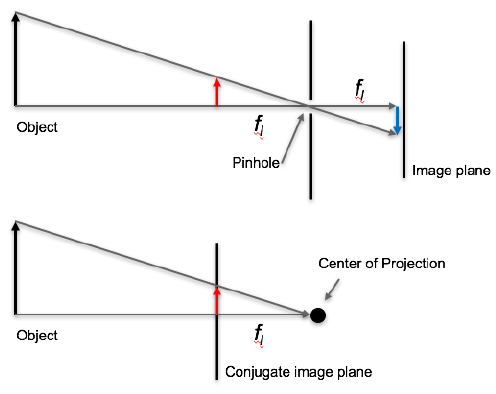
\includegraphics[width=0.7\textwidth]{projection}
	\caption{Simple projection imaging ray diagram.}
	\label{fig:projection}
\end{figure}

Analyzing the relationships between points in the ray diagram of fig. \ref{fig:projection}, we see in fig. \ref{fig:proj_relations} there is a simple relationship for points in a projection.

\begin{figure}[ht]
	\centering
	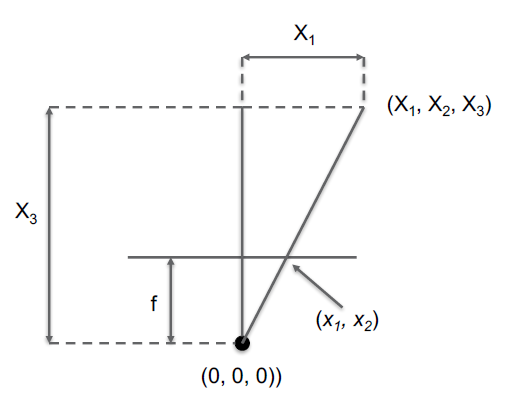
\includegraphics[width=0.6\textwidth]{proj_relations}
	\caption{A projection image and arbitrary object plane of focal distance, f.}
	\label{fig:proj_relations}
\end{figure}

Geometrically, we have 
\begin{align*}
\frac{f}{X_3} &= \frac{x_1}{X_1} \\
x_1 &= f\frac{X_1}{X_3} \\
\text{and by a similar argument,} \\
x_2 &= f\frac{X_2}{X_3}
\end{align*}

Therefore, the camera coordinates, $(X_1, X_2, X_3)$ are related to the canonical image coordinates, $(x_1, x_2)$ as

\begin{equation}
	\begin{bmatrix}
		x_1 \\
		x_2
	\end{bmatrix}
	=
	\begin{bmatrix}
		f & 0 \\
		0 & f \\
	\end{bmatrix}
	\begin{bmatrix}
		X_1 \\
		X_2
	\end{bmatrix}
	\frac{1}{X_3}
\end{equation}

However, this relationship is non-linear and we can do this another way. By finding a relationship in \textit{homogeneous} coordinates, we arrive at a linear relationship

\begin{equation}
	\vec{x} = 
	\begin{bmatrix}
		x_1 \\
		x_2 \\
		x_3
	\end{bmatrix}
	=
	\begin{bmatrix}
		f & 0 & 0 & 0 \\
		0 & f & 0 & 0 \\
		0 & 0 & 1 & 0 
	\end{bmatrix}
	\begin{bmatrix}
		X_1 \\
		X_2 \\
		X_3 \\
		1
	\end{bmatrix}
\end{equation}

where the canonical coordinates of the projection point, $\vec{x}$ are found as $x_1/x_3$ and $x_2/x_3$.

Thus, while in Euclidean geometry, a point in N-D space is described by an N-D vector, in projective geometry, a point in N-D space is described by an (N+1)-D vector. The last coordinate, $k$ is a multiplier of the first N coordinates. Then, a point can be scaled by $k$ as $(k*rows, k*cols, k)$, a homogeneous vector.

\paragraph{Fact:} Given a set of world points known to lie on a plane, there exists a matrix, $H$, that maps the $(row, col)$ image points in one camera to the the $(row, col)$ image points in another camera. Mathematically,

\begin{equation} \label{eq:hmap}
\vec{v} = H\vec{x}.
\end{equation}

For our purpose of correcting perspective distortion, we take $\vec{x}$ to be a homogeneous vector of a point in the distorted image, $\vec{v}$ to be a homogeneous vector of the same point in the corrected image, and seek a matrix $H$ that maps lines converging at infinity to parallel lines in the Euclidean plane. 

The process of perspective distortion correction will consist of choosing a set of points in a distorted image that lie on a plane, although not all on the same line. We will choose 20 points and two lines (10 points per line). Then, we will define 20 points, again in two lines, of which to map each pixel index. 

\pagebreak

\paragraph{Procedure} Using GIMP and the mouse cursor, I selected 10 points on successive corners of the upper windows in the image shown in fig. \ref{fig:distorted} and 10 more points on the lower windows. Then choosing a relatively arbitrary range of values along the \textit{col} dimension, and two constant values of \textit{row}, I generated a set of 20 points in the horizontal direction, of which to map the original points into a corrected image. 

\begin{figure}[ht]
	\centering
	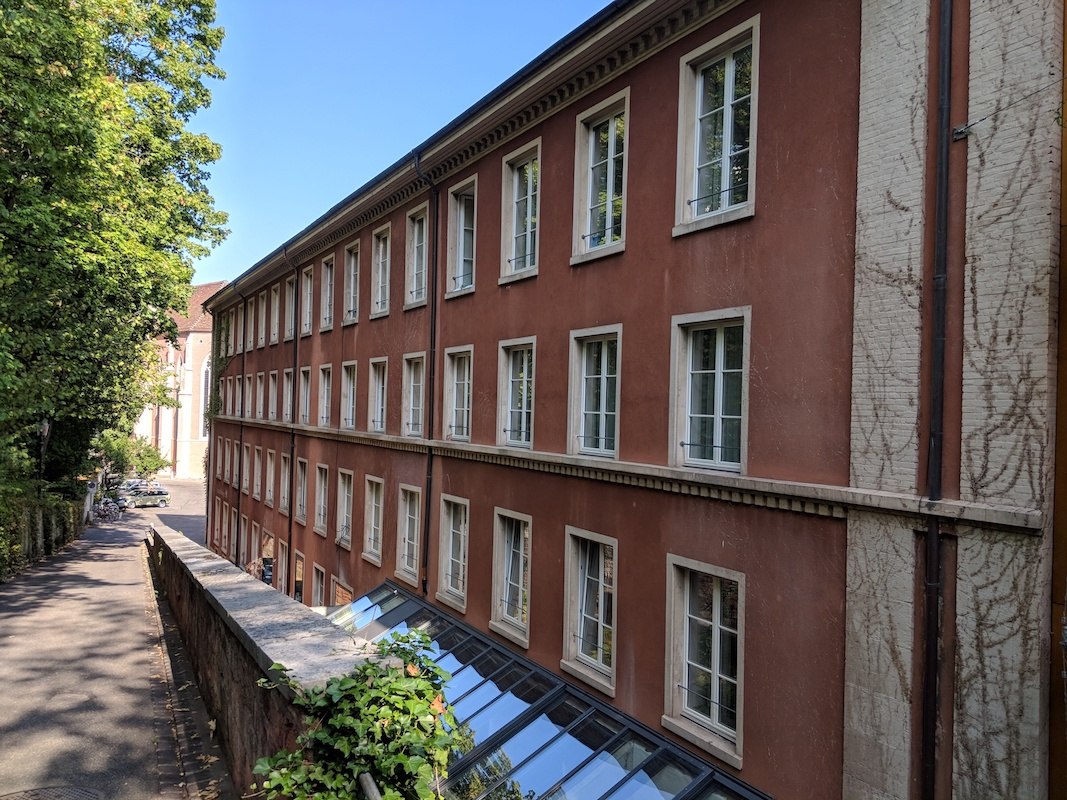
\includegraphics[width=0.9\textwidth]{PC_test_2}
	\caption{Distorted image to be corrected.}
	\label{fig:distorted}
\end{figure}

Thus, the mapping for the first line is

\begin{equation}
	\begin{bmatrix}
		750 & 215 \\
		675 & 235 \\
		625 & 250 \\
		575 & 265 \\
		535 & 275 \\
		500 & 285 \\
		475 & 295 \\
		445 & 300 \\
		425 & 305 \\
		405 & 315
	\end{bmatrix}
	\longrightarrow
	\begin{bmatrix}
		750 & 305 \\
		711.67 & 305 \\
		673.33 & 305 \\
		635 & 305 \\
		596.67 & 305 \\
		558.33 & 305 \\
		520 & 305 \\
		481.67 & 305 \\
		443.33 & 305 \\
		405 & 305
	\end{bmatrix}
\end{equation}

and for the second line,

\begin{equation}
	\begin{bmatrix}
		745 & 575 \\
		670 & 555 \\
		615 & 540 \\
		565 & 525 \\
		530 & 515 \\
		495 & 505 \\
		468 & 500 \\
		440 & 495 \\
		420 & 488 \\
		400 & 483
	\end{bmatrix}
	\longrightarrow
	\begin{bmatrix}
		750 & 475 \\
		711.67 & 475 \\
		673.33 & 475 \\
		635 & 475 \\
		596.67 & 475 \\
		558.33 & 475 \\
		520 & 475 \\
		481.67 & 475 \\
		443.33 & 475 \\
		405 & 475
	\end{bmatrix}
\end{equation}

Considering a point in the distorted image to be $(c,d)$ and a point in the corrected image, $(a,b)$, the above relation can be expressed

\begin{align*}
	(c_1,d_1) &= (a_1,b_1) \\
	(c_2,d_2) &= (a_2,b_2) \\
	\ldots \\
	(c_{20},d_{20}) &= (a_{20},b_{20})
\end{align*}

Now, the relationship we need to find is

\begin{equation} \label{eq:H}
	\begin{bmatrix}
		v_1 \\
		v_2 \\
		v_3
	\end{bmatrix}
	=
	\begin{bmatrix}
		h_11 & h_12 & h_13 \\
		h_21 & h_22 & h_23 \\
		h_31 & h_32 & 1
	\end{bmatrix}
	\begin{bmatrix}
		c \\
		d \\
		1
	\end{bmatrix} 
	\text{and}
	\begin{bmatrix}
		a \\
		b
	\end{bmatrix}
	=
	\begin{bmatrix}
		v_1/v_3 \\
		v_2/v_3
	\end{bmatrix}
\end{equation}

Solving for $v_1/v_3$ and $v_2/v_3$ in \ref{eq:H}, we find

\begin{align*}
a &= \frac{h_{11} c + h_{12} d + h_{13}}{h_{31} c + h_{32} d + 1} \\
b &= \frac{h_{21} c + h_{22} d + h_{23}}{h_{31} c + h_{32} d + 1}
\end{align*}

which can also be written in matrix form as 

\begin{equation} \label{eq:mapping}
	\begin{bmatrix}
		c & d & 1 & 0 & 0 & 0 & -ac & -ad \\
		0 & 0 & 0 & c & d & 1 & -bc & -bd
	\end{bmatrix}
	\begin{bmatrix}
		h_{11} \\
		h_{12} \\
		h_{13} \\
		h_{21} \\
		h_{22} \\
		h_{23} \\
		h_{31} \\
		h_{32}
	\end{bmatrix}
	=
	\begin{bmatrix}
		a \\
		b
	\end{bmatrix}
\end{equation}

\pagebreak

The Python procedure for this process goes as follows. First, we define a list of pixel coordinate points in the distorted image, \verb|inputPoints| and the points to map into, \verb|outputPoints|. Then, we build the left-hand side of \eqref{eq:mapping}, constructing a [40, 8] matrix, \verb|mapping| (two rows for each point). Using the same method as we did in the linear regression problem, we find the pseudo inverse, \verb|mapping_inv = np.linalg.inv(mapping.T.dot(mapping)).dot(mapping.T)|. Reshaping the set of output points into a [40, 1] vector allows us to calculate $H = mapping_{inv} \cdot outputPoints$ ([9, 1]). We then append $1$ to the end, and reshape into a [3, 3] matrix.

At this point, we are ready to remap every pixel in the distorted image to generate a corrected image. We initialize a new \verb|numpy| array to be the same dimensions as the distorted image and begin stepping over each pixel. The method, now, is to compute $\vec{v} = H^{-1} \cdot \vec{p}$, where $\vec{p}$ is the pixel index of the corrected image, and $[a,b] = [v_1/v_3, v_2/v_3]$

We then check to verify that $[a,b]$ is within the bounds of the distorted image dimensions and perform a bilinear interpolation to find the RGB intensity value for the current pixel in the corrected image.

\pagebreak

\begin{figure}[ht]
	\centering
	\begin{subfigure}[h]{0.8\textwidth}
		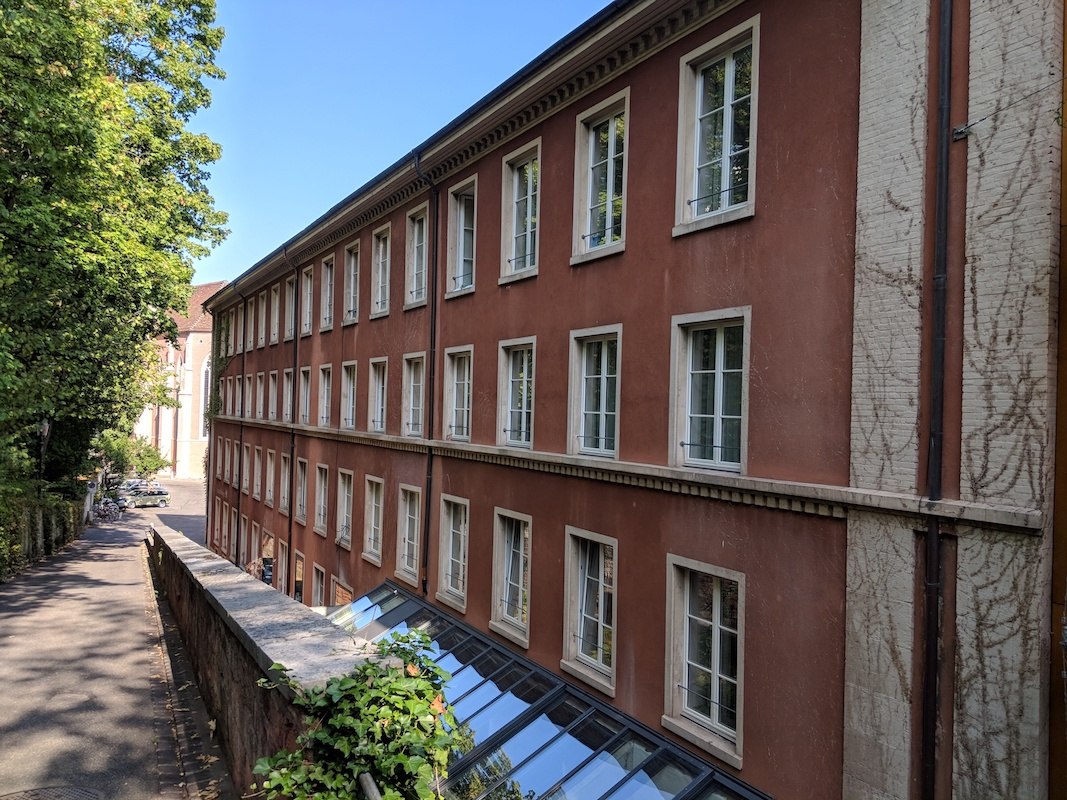
\includegraphics[width=\textwidth]{PC_test_2}
		\caption{Original "distorted" image.}
		\label{fig:original}
	\end{subfigure}
	\par\medskip
	\begin{subfigure}[h]{0.8\textwidth}
		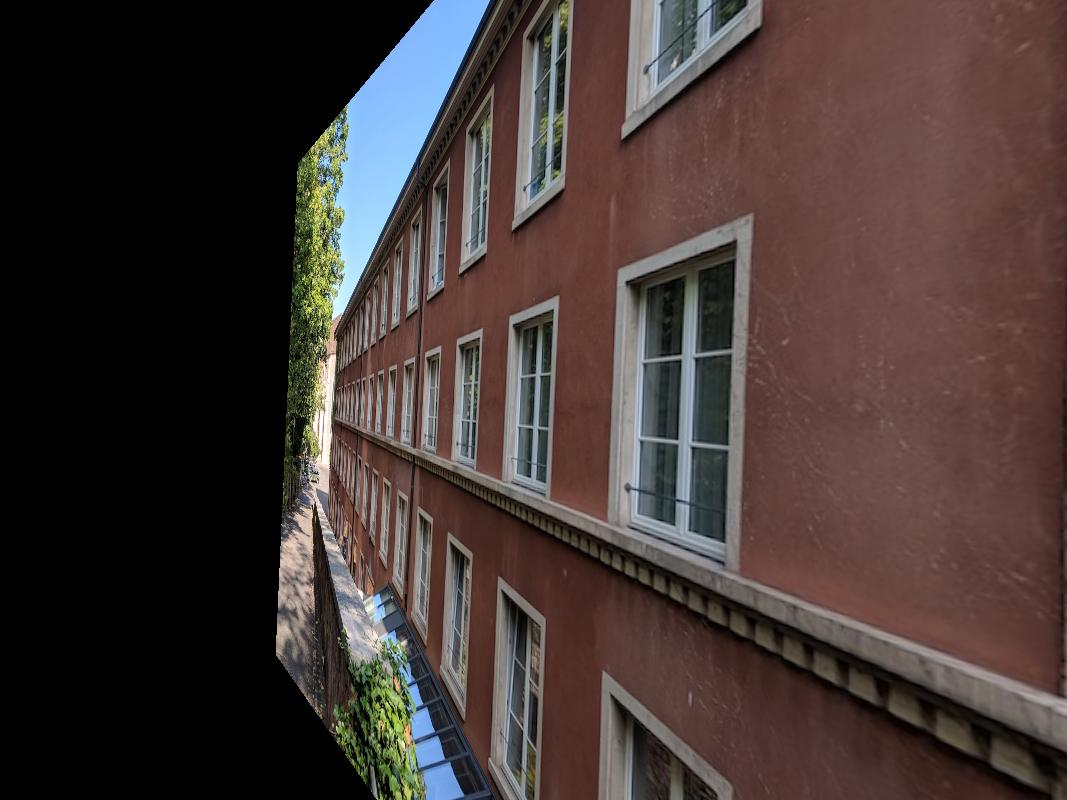
\includegraphics[width=\textwidth]{out1}
		\caption{Corrected image.}
		\label{fig:corrected}
	\end{subfigure}
	\caption{Perspective distortion correction.}
	\label{fig:correction}
\end{figure}

\clearpage

Notice how the image gets increasingly blurry toward the left-hand side. This is due to the interpolation in this region. The mapping we attempted, tried to squeeze the right-hand side down, while stretching the left-hand side up. The mapping function also sets pixels to black if they are out of range of the original image, so there are large black triangles, where the perspective correction had no data to interpolate from for those regions. It may look better if the image was cropped, or a different set of output points was chosen. Unfortunately, this method also does not accommodate points that do not lie in the same plane as those being remapped very well. Notice the vines at the bottom left of the original image and how they were stretched in processing. This makes sense if we imagine the vines do live in the same plane as the side of the building, like graffiti painted on. Then, the vines appear to spread over a large horizontal length of the wall and when mapped, appear stretched.

Choosing a different set of points in the output image, the picture in fig. \ref{fig:map2} was generated. Notice how it is possible to effectively zoom in using this remapping method.

\begin{figure}[ht]
	\centering
	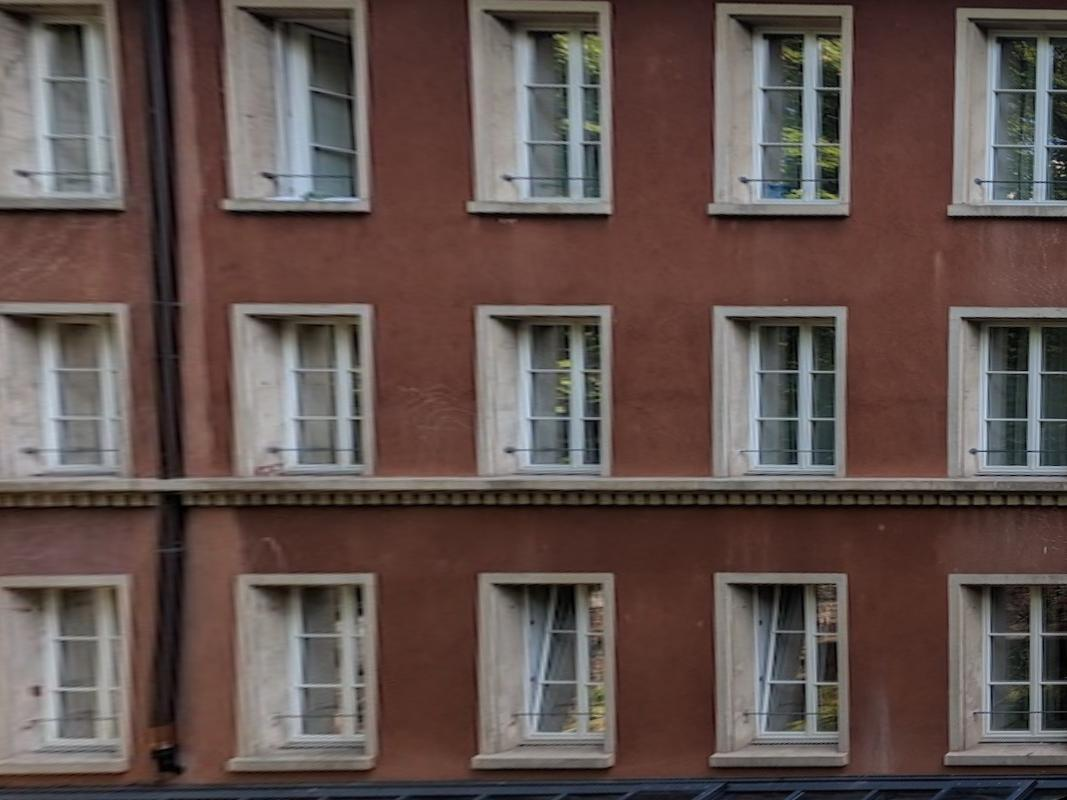
\includegraphics[width=0.8\textwidth]{out2}
	\caption{A different mapping.}
	\label{fig:map2}
\end{figure}

\pagebreak

\section{Motion Tracking}
For "motion tracking" we will really be doing some motion estimation. By slicing up an image into small "chunks" or "blocks", we can perform a localized search for similar blocks within a specified range. 

\begin{figure}[ht]
	\centering
	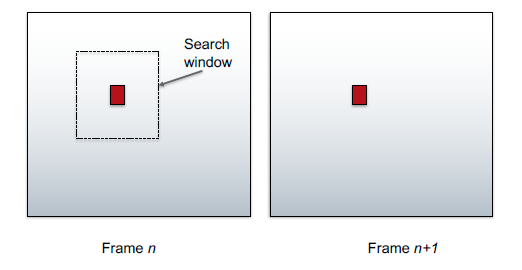
\includegraphics[width=0.8\textwidth]{motion_search}
	\caption{Cartoon representation of a motion estimation localized search.}
	\label{fig:search}
\end{figure}

We consider two frames of a video, $n$ and $n+1$. By looping over blocks of pixels in frame $n+1$, we can perform the search to find the minimum MSE for a nearby block and select that block to be used as a prediction of the motion that occurred.

Starting with a pixel index and search range, the algorithm to do the motion estimation essentially slides the block into every possible position within the search range and calculates the MSE at that location. The location, MSE, and predicted block are returned, so a prediction image can be generated. 

\pagebreak

\begin{figure}[ht]
	\centering
	\begin{subfigure}[h]{0.7\textwidth}
		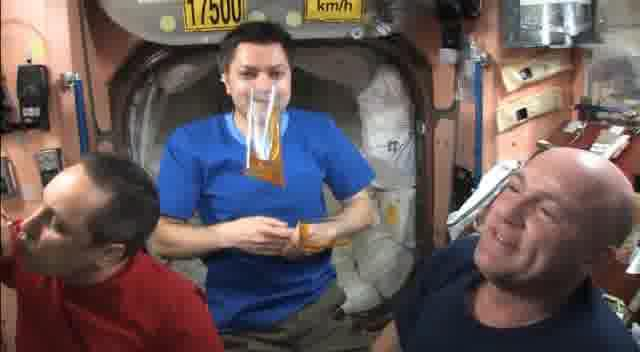
\includegraphics[width=\textwidth]{xi01}
		\caption{frame $n$}
	\end{subfigure}
	\par\medskip
	\begin{subfigure}[h]{0.7\textwidth}
		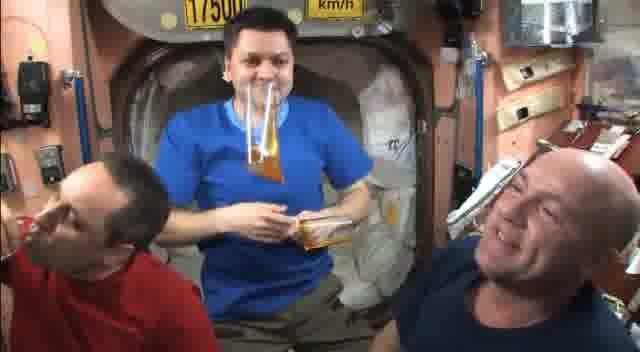
\includegraphics[width=\textwidth]{xi02}
		\caption{frame $n+1$}
	\end{subfigure}
	\caption{Two frames of a video taken in the ISS.}
	\label{fig:two_frames}
\end{figure}

The two frames we will use for motion estimation are shown in fig. \ref{fig:two_frames}. First, the result using MSE is shown.

\begin{figure}[ht]
	\centering
	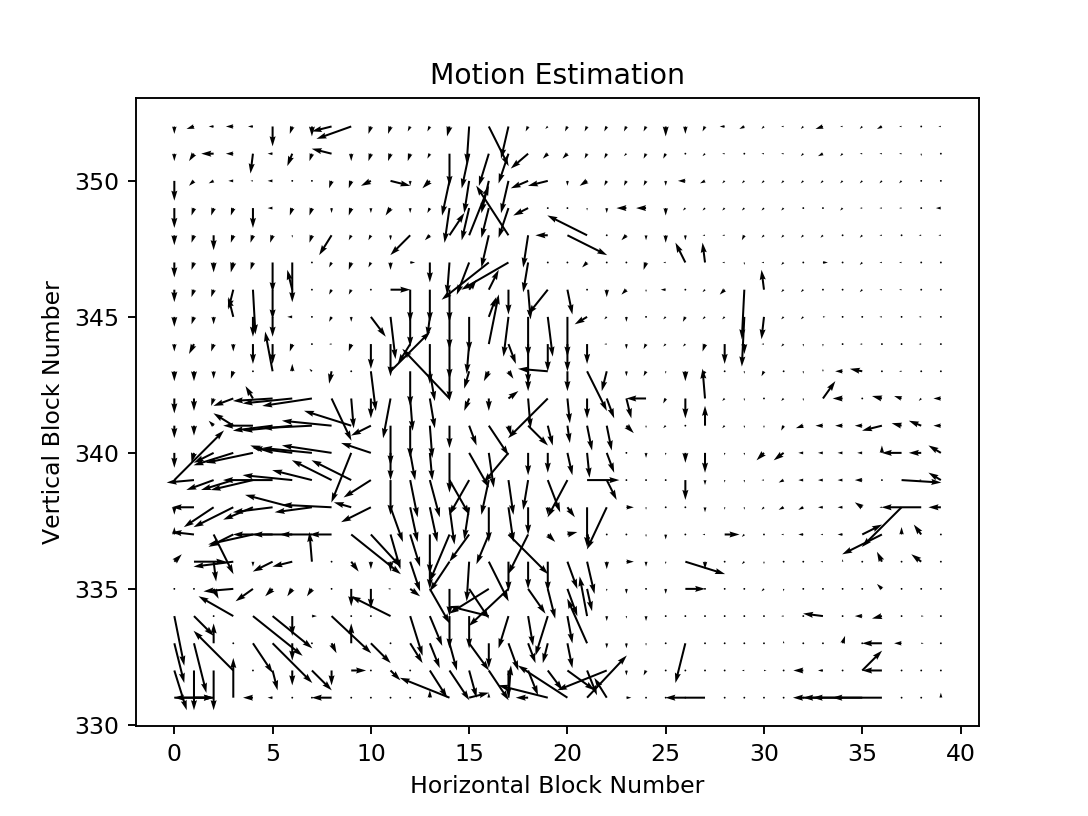
\includegraphics[width=0.7\textwidth]{vector_field}
	\caption{The relative direction of motion for each block analyzed using MSE, represented as a vector field.}
	\label{fig:vector}
\end{figure}

Looking closely at fig. \ref{fig:vector}, you can almost see the shape of each person in the frame and their slight motion between the two frames. The predicted motion determined by the search algorithm is shown in fig. \ref{fig:predicted}.

\pagebreak

\begin{figure}[ht]
	\centering
	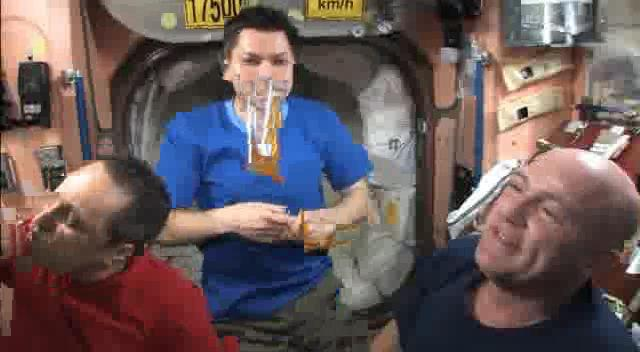
\includegraphics[width=0.7\textwidth]{predicted}
	\caption{Predicted motion for search using MSE.}
	\label{fig:predicted}
\end{figure}

It is obvious that this search method isn't perfect, because there are some artifacts of the process around their eyes and especially near the mouth of the man in the center of the frame. Regardless, for an estimation, it isn't bad.

\pagebreak

Next, we look at the same process, but for mean absolute error (MAE). 

\begin{figure}[ht]
	\centering
	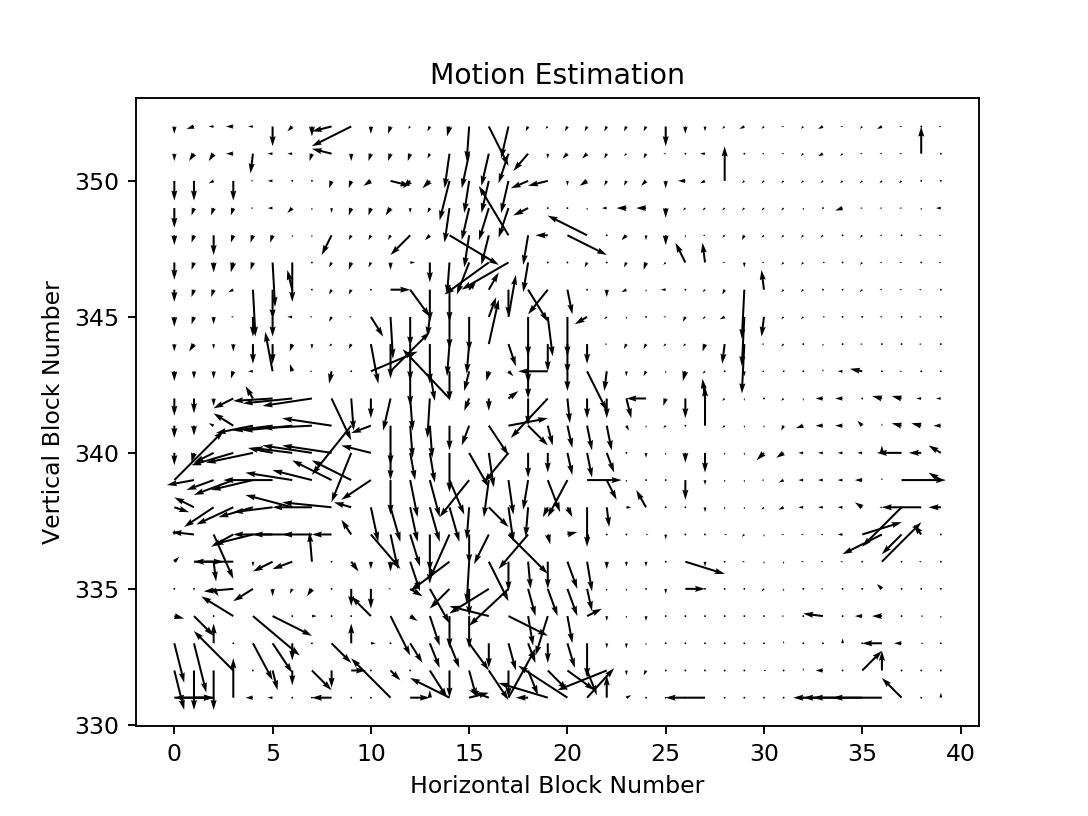
\includegraphics[width=0.7\textwidth]{vector_field1}
	\caption{The relative direction of motion for each block analyzed using MAE, represented as a vector field.}
	\label{fig:vector1}
\end{figure}

Notice in fig. \ref{fig:vector1} that there are a few vectors with larger magnitude than in fig. \ref{fig:vector}. This is because small deviations are not scaled down in the MAE. Only the absolute difference is considered, so this version of the algorithm is more sensitive to changes, at the expense of possibly detecting noise more frequently. The predicted image is also shown in fig. \ref{fig:predicted1}, but there really are not any noticeable differences compared to the MSE version.

\begin{figure}[ht]
	\centering
	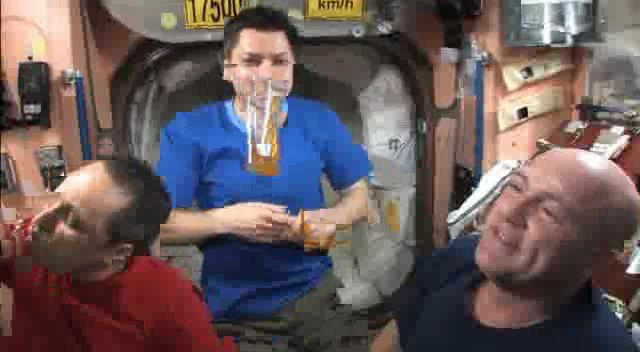
\includegraphics[width=0.7\textwidth]{predicted1}
	\caption{Predicted motion for search using MAE.}
	\label{fig:predicted1}
\end{figure}

\pagebreak

\section{Conclusion}
Projection in linear algebra is a difficult concept! the transformations we used in this lab were very hard to follow and it was difficult to understand why we were computing some of these. Despite that, this was a really cool introduction to perspective correction and the idea of distortion manipulation and projection theory. I found this lab really challenging, but interesting. The motion detection algorithm was a lot easier to follow. 

\pagebreak

\section{Appendix}
\subsection{A: Linear Regression}
\begin{lstlisting}[language=Python]
import numpy as np

def linReg(A, C):
    # compute pseudo inverse matrix
    A_p = np.linalg.inv(A.T.dot(A)).dot(A.T)
    #print(f'A_p = {A_p}\n')
    # compute weighting coefficient vector
    x = A_p.dot(C)
    #print(f'x = {x}\n')
    # compute mapped values
    v = A.dot(x)
    #print(f'v = {v}\n')
    # compute mean-squared-error of solutions
    mse = (abs(v-C))**2
    #print(f'MSE = {mse}')
    
    return x, v, A_p, mse
\end{lstlisting}

\pagebreak

\subsection{B: Perspective Distortion Correction}
\begin{lstlisting}[language=Python]
import numpy as np
import sys
import bilinear_interp as interp

def distortion_correction(imageIn, inPoints, outPoints):
    # build remapping matrix for calculation of H
    mapping = np.zeros([0, 8])
    for row in range(20):
        ip1 = inPoints[row, 0]
        ip2 = inPoints[row, 1]
        op1 = outPoints[row, 0]
        op2 = outPoints[row, 1]
        arr = np.asarray([[ip1, ip2, 1, 0, 0, 0, -op1*ip1, -op1*ip2],
                          [0, 0, 0, ip1, ip2, 1, -op2*ip1, -op2*ip2]])
        mapping = np.append(mapping, arr, axis=0)
    #print(f'mapping = {mapping}\n shape(mapping) = {np.shape(mapping)}\n')

    # calculate pseudo inverse to find H
    mapping_inv = np.linalg.inv(mapping.T.dot(mapping)).dot(mapping.T)
    outPoints = np.reshape(outPoints, [40, 1])
    #print(f'outPoints = {outPoints}\n')

    # find H by taking the dot product of H* and output points
    H = mapping_inv.dot(outPoints)
    #print(f'shape(H) = {np.shape(H)}')
    H = np.append(H, 1)
    H = np.reshape(H, [3,3])
    #print(f'H = {H}\n')
    H_inv = np.linalg.inv(H)

    # correct distortion of perspective image
    corrImage = np.zeros([np.shape(imageIn)[0], np.shape(imageIn)[1], 3])
    print('remapping pixels...')
    # take the dot product of H with each pixel in distorted image
    for y in range(np.shape(corrImage)[0]):
        for x in range(np.shape(corrImage)[1]):
            p = [x, y, 1]
            v = H_inv.dot(p)
            # calculate points in distorted image corresponding to corrected pixels
            map = [v[0]/v[2], v[1]/v[2]]
            # interpolate to find real pixel values
            corrImage[y, x, :] = interp.bilinear_interp(map[0], map[1], imageIn)
        # print progress bar
        progress = int(y*100/np.shape(corrImage)[0])
        sys.stdout.write('{0}% complete...\r'.format(progress))
        sys.stdout.flush()
    print('\n')

    return corrImage, H, imageIn
\end{lstlisting}

\pagebreak

\subsection{C: Motion Detection}
\begin{lstlisting}[language=Python]
import me_method as me
import numpy as np
import matplotlib.pyplot as plt
from PIL import Image
import sys

def detect_motion(frame1, frame2, blockSize):
    im1 = np.asarray(Image.open(frame1))
    im2 = np.asarray(Image.open(frame2))
    im1_bw = np.asarray(Image.open(frame1).convert('L'), np.float)
    im2_bw = np.asarray(Image.open(frame2).convert('L'), np.float)

    rows = np.shape(im2)[0]
    cols = np.shape(im2)[1]
    blockSize = 16

    predicted_image = np.zeros([rows, cols, 3], np.uint8)
    MSE = np.zeros([rows, cols], np.float)
    vectorCount = int((rows/blockSize) * (cols/blockSize))
    U = np.zeros(vectorCount)
    V = np.zeros(vectorCount)
    X = np.zeros(vectorCount)
    Y = np.zeros(vectorCount)
    currIndex = 0
    # loop over blocks
    print('Estimating motion ... \n')
    for row in range(0, rows, blockSize):
        for col in range(0, cols, blockSize):
            block = im2_bw[row:row + blockSize, col:col + blockSize]
            motion_estimation = me.motion_match(row, col, 20, block, im1_bw, im1)
            predicted_image[row:row + blockSize, col:col + blockSize] = motion_estimation[0]
            MSE[row, col] = motion_estimation[1]
            U[currIndex] = motion_estimation[3]
            V[currIndex] = -motion_estimation[2]
            X[currIndex] = int(col/blockSize)
            Y[currIndex] = rows - int(row/blockSize)
            currIndex += 1
        progress = int((row*100)/rows)
        sys.stdout.write('{0}% complete...\r'.format(progress))
        sys.stdout.flush()
    print('\n')
    Image.fromarray(predicted_image.astype(np.uint8)).save('predicted.jpg')
    plt.figure(dpi=170)
    plt.quiver(X, Y, U, V)
    plt.title("Motion Estimation")
    plt.xlabel("Horizontal Block Number")
    plt.ylabel("Vertical Block Number")
    plt.ion()
    plt.savefig('vector_field.png')

    return 0
\end{lstlisting}

\pagebreak

\subsection{D: Main}
\begin{lstlisting}[language=Python]
# Created by Andrew Teta
# 2019/02/13
# ECEN 4532 DSP Lab 3
# Perspective Transformations and Motion Tracking

import numpy as np
from PIL import Image
import sys
import lab3_funcs as lf

A = np.asarray([[1,8,3,65.66],
                [-46,-98,108,-1763.1],
                [5,12,-9,195.2],
                [63,345,-27,3625],
                [23,78,45,716.9],
                [-12,56,-8,339],
                [1,34,78,-25.5],
                [56,123,-5,1677.1]])
C = A[:,3]
A = A[:,0:-1]
#print(f'A = {A}\n')
#print(f'C = {C}\n')

# calculate linear regression
linear_regression = lf.linReg(A, C)
print(f'x = {linear_regression[0]}\n')
print(f'MSE = {linear_regression[3]}\n')

# build perspective lines to be corrected
inputPoints = np.asarray([[750, 215],
                          [675, 235],
                          [625, 250],
                          [575, 265],
                          [535, 275],
                          [500, 285],
                          [475, 295],
                          [445, 300],
                          [425, 305],
                          [405, 315],
                          [745, 575],
                          [670, 555],
                          [615, 540],
                          [565, 525],
                          [530, 515],
                          [495, 505],
                          [468, 500],
                          [440, 495],
                          [420, 488],
                          [400, 483]])
#print(f'inputPoints = {inputPoints}\n')

# build output lines
outputLine1 = np.zeros([10, 2])
outputLine2 = np.zeros([10, 2])
line1 = np.linspace(750, 405, 10)
line2 = np.linspace(750, 405, 10)
for i in range(10):
    outputLine1[i] = [line1[i], 305]
    outputLine2[i] = [line2[i], 475]

# combine output lines into one vector of points
outputPoints = np.append(outputLine1, outputLine2, axis=0)
#print(f'outputPoints = {outputPoints}\n shape(outputPoints) = {np.shape(outputPoints)}\n')

# correct distortion
distImage = Image.open('PC_test_2.jpg')
distImage = np.asarray(distImage)
perspective_correct = lf.distortion_correction(distImage, inputPoints, outputPoints)

# display and save image
Image.fromarray(perspective_correct[0].astype(np.uint8)).show()
Image.fromarray(perspective_correct[0].astype(np.uint8)).save('out1.jpg')

line = np.linspace(1080, 0, 10)
y1 = 215
y2 = 575
# build output lines
outputLine1 = np.zeros([10, 2])
outputLine2 = np.zeros([10, 2])
for i in range(10):
    outputLine1[i] = [line[i], y1]
    outputLine2[i] = [line[i], y2]
# combine output lines into one vector of points
outputPoints1 = np.append(outputLine1, outputLine2, axis=0)

# correct distortion
perspective_correct1 = lf.distortion_correction(distImage, inputPoints, outputPoints1)
# display and save image
Image.fromarray(perspective_correct1[0].astype(np.uint8)).show()
Image.fromarray(perspective_correct1[0].astype(np.uint8)).save('out2.jpg')

# Motion Tracking #
lf.detect_motion('xi01.jpg', 'xi02.jpg', 16)
lf.detect_motion_mae('xi01.jpg', 'xi02.jpg', 16)

print('done')
\end{lstlisting}

\end{document}